\documentclass[
  twoside,
  11pt, a4paper,
  footinclude=true,
  headinclude=true,
  cleardoublepage=empty
]{scrreprt}

\usepackage{lipsum}
\usepackage[utf8]{inputenc}
\usepackage[ngerman,english]{babel}
\usepackage{amsmath}
\usepackage{amsthm}
\usepackage{graphicx}
\usepackage{listings}
\usepackage{lmodern}
\usepackage{float}
\usepackage{sidecap}
\usepackage{todonotes}
\usepackage{siunitx}
\usepackage{acronym}
\usepackage{setspace}
\usepackage[customcolors]{hf-tikz}
\usepackage{url}
\usepackage{csquotes}
\usepackage[T1]{fontenc}
\graphicspath{ {images/} }

\begin{document}

\begin{titlepage}
    \begin{center}
        \Huge
        \textbf{Feasibility Study of Real Time Path Tracing}
        
        \vspace{0.5cm}

        \LARGE
        \textit{Or:} How Much Noise Is Too Much?
        
        \vspace{1.5cm}
        
        \textbf{Sven-Hendrik Haase}
        
        \vfill
        
        A thesis presented for the degree of\\
        \emph{Bachelor of Computer Science}
        
        \vspace{0.8cm}
        
        
\includegraphics[width=0.4\textwidth]{frontbackmatter/logo_uhh.jpg}
        
        % I was not allowed to use the old logo :( But I have much like it so I'm
        % keeping this here.
        %
\includegraphics[width=0.4\textwidth]{frontbackmatter/uni-siegel.png}
        
        \Large
        Department of Informatics\\
        University of Hamburg\\
        Germany\\
        2015-20-08

        \vspace{0.8cm}

        \large
        Primary Supervisor: Prof. Dr. rer. nat. Leonie \textsc{Dreschler-Fischer}\\
        Secondary Supervisor: Prof. Dr. Thomas \textsc{Ludwig}
        
    \end{center}
\end{titlepage}


\chapter*{Abstract}
\onehalfspace
This study aims to investigate the viability of a physically-based technique called
\textbf{path tracing} in lieu of or in corporation with classical techniques in interactive media
such as video games and visual effects tools.

Real time path tracing has been prohibitively expensive in regards to computational complexity.
However, modern \acs{gpu}s and even \acs{cpu}s have finally gotten fast enough for real time path
tracing to become a viable alternative to traditional real time approaches to rendering.  Based on
that assumption, this thesis presents the idea, algorithm and complexity behind path tracing in the
first part and extrapolates feasibility and suitability of real time path tracing on consumer
hardware according to the current state of technology and trends in the second part.

As part of the research, the author has implemented a path tracing 3D engine in modern C++ in order
to empirically test the assumptions made in this thesis. The study found path tracing to be a
viable rendering technique for average commodity hardware in approximately 4 years.
\singlespace

\chapter*{Acknowledgments}
\doublespacing
I would like to express my sincere gratitude to the teachers throughout school and university for
the knowledge they've passed on.

I thank my friends for the laughs, horrible mistakes and awesome successes we shared with
one another.

Furthermore, none of this would have been possible without the incredible efforts and love of my
parents who have supported me throughout the years and enabled me to live a carefree life until I
was ready to fend for myself.

Lastly, but certainly not least, I would like to declare my gratefulness to Alisa, whose endless love
has given my life a new meaning.

\singlespace

\clearpage
\vspace*{\fill}
\thispagestyle{empty} % suppress showing of page number
\begin{quotation}
    \em
    We all make choices in life, but in the end, our choices make us.

    \medskip
    \raggedleft
    Andrew Ryan
\end{quotation}
\vspace*{\fill}

\tableofcontents

\chapter*{Acronyms}
\begin{acronym}
    \acro{aabb}[AABB]{axis-aligned bounding box}
    \acro{ao}[AO]{ambient occlusion}
    \acro{brdf}[BRDF]{bidirectional reflection distribution function}
    \acro{bsp}[BSP]{binary space partitioning}
    \acro{cpu}[CPU]{central processing unit}
    \acro{csg}[CSG]{constructive solid geometry}
    \acro{fps}[FPS]{frames per second}
    \acro{gi}[GI]{global illumination}
    \acro{gpu}[GPU]{graphics processing unit}
    \acro{hdr}[HDR]{high dynamic range}
    \acro{mlt}[MLT]{Metropolis light transport}
    \acro{pbr}[PBR]{physically based rendering}
    \acro{rt}[RT]{real time}
    \acro{rgb}[RGB]{red-green-blue}
    \acro{simd}[SIMD]{single instruction multiple data}
    \acro{spp}[SPP]{samples per pixel}
    \acro{ssao}[SSAO]{screen-space ambient occlusion}
\end{acronym}

\chapter{Introduction}
As part of the quest for ever-improving game graphics, researchers, graphics hardware developers
and video game developers alike have been coming up with more and more convoluted and technically
challenging ways of improving the graphics in interactive media such as games and visualizations in
order to give users a deeper sense of immersion or to provide special effects artists with faster
feedback.

While rendering techniques are currently shifting from the traditional fixed pipeline approach
towards the new, fully programmable approach that lets developers implement deferred renderers that
can more closely mimic reality by using multiple combined shading and lighting algorithms and
rendering the scene multiple times for different buffers, the fundamental concept of
rasterization-based rendering has largely remained the same.

The real world photon-collecting approach that actual cameras use has so far not been adopted for
interactive media by the industry in any capacity because the computational cost has historically
been prohibitively expensive. It is, however, used extensively (and has been in use since decades)
for offline, non-interactive rendering of computer-generated movies and visualizations of
scientific simulations.

This study assumes that the next logical step for the industry will be to adopt this method for
real time media as well. For the purpose of this thesis, a renderer is considered
\textit{real time} when it manages to render a frame within \(16.67ms\) since that equals 60
\ac{fps} which is
the current de facto standard refresh rate for most available computer screens. Conversely, a
renderer is called \textit{offline} when it is not designed for interactive rendering which usually
means that it will renderer an image or a batch of images over the course of a few days. The
differences of real time and offline path tracing renderers will be explained in the next chapter.

\section{Motivation}
Real time path tracing (and physically based rendering in general) offers many
benefits over traditional real time rendering methods such as better visuals
and simpler implementation but also allows for completely new types of graphics
such as realistic caustics \cite{wiki:caustics} and even light dispersion
\cite{wiki:dispersion} (using a prism, for instance) since path tracers might simulate wavelengths
instead of plain \ac{rgb} colors. Modern video games tend
to rely on a growing number of tricks to keep them visually appealing as the
consumer grows more demanding. They're called \textit{tricks} in this study
because they merely trick the beholder into seeing something that appears to be
physically accurate when it is, in fact, not the result of a physically-based
calculation and as such this study aims to keep tricks and emergent phenomena
separated by language. Some notable tricks include \ac{ssao}
\cite{wiki:ssao}, motion blur \cite{wiki:motion-blur}, lens flares
\cite{wiki:lens-flare}, chromatic aberration \cite{wiki:chromatic-aberration},
depth of field \cite{wiki:depth-of-field} and light mapping \cite{wiki:lightmap}.

\chapter{Real Time Path Tracing Explained}
This chapter will explain the concepts, mathematics, physics and algorithms behind path tracing,
how real time path tracing differs from offline path tracing and the trade-offs made to achieve
acceptable performance. It will also explain how path tracing differs from rasterization and other
\ac{gi} techniques.

\section{Physically Based Approach}
In our physical world, we see pictures because our eyes collect photons emitted by light
sources which then bounce around various surfaces until they eventually hit our eyes'
photoreceptor cells. On every bounce, a bit of light is absorbed which is why light loses intensity
when it bounces. Some surfaces absorb a particular band of wavelengths of the light when it bounces
which we perceive as a change in the light's color. Cameras work exactly like this as far as
collection of photons is concerned.

This physical approach would be extremely wasteful and
computationally complex to simulate, however, since most photons never reach an observer. Consider,
for instance, that only an extremely small percentage of all the photons sent by the Sun actually
reach Earth and an even smaller percentage of those are ever observed (although photons
don't have to be observed to have a physical effect, of course). Since we only care for photons that
are relevant to the image that we are trying to render, it makes more sense to use
\emph{backwards ray tracing} in which rays (which simulate streams of photons) are shot from the
observer into the scene for every sensor. It is called \textit{backwards} because the rays go
the reverse direction compared to their physical counterparts.

This is efficient since we usually only care about a
single observer (the scene camera) for which we will trace every single ray that it can possibly
perceive. In computer graphics terms, we will trace a ray for every pixel of the camera (and for
now we will assume that the viewport is exactly the same resolution as the camera simplicity's
sake). For every ray, we check for intersections with geometry and then either bounce a few more
times or shoot directly towards a light. We might do this multiple times per pixel to improve image
quality. This is called \emph{sampling}. The more iterations we spend on sampling, the better the
quality of our image becomes. This is called \emph{converging}.
There are a few approaches that improve on this such as bidirectional path tracing
\cite{techreport:pbr} and the \ac{mlt} \cite{inproceedings:metropolis}.

\section{Theoretical Basis}
\subsection{The Rendering Equation}
The fundamental problem solved by path tracing is the \emph{rendering equation} originally
described by James Kajiya \cite{inproceedings:pathtracing}. This thesis uses the form from
Wikipedia \cite{wiki:rendering-equation} since the author considers it easier to read:

\[
        L_{\text{o}}(\mathbf x,\, \omega_{\text{o}},\, \lambda,\, t) \,=
        \, L_{\text{e}}(\mathbf x,\, \omega_{\text{o}},\, \lambda,\, t) \ +
        \, \int_\Omega f_{\text{r}}(\mathbf x,\, \omega_{\text{i}},\ \omega_{\text{o}},\, \lambda,\, t)
        \, L_{\text{i}}(\mathbf x,\, \omega_{\text{i}},\, \lambda,\, t)\,
        (\omega_{\text{i}}\,\cdot\,\mathbf n)\, \operatorname d \omega_{\text{i}}
\]

For our purposes, this can be simplified by removing the time and wavelength components which we
will not make use of:

\[
        L_{\text{o}}(\mathbf x,\, \omega_{\text{o}}) \,=
        \, L_{\text{e}}(\mathbf x,\, \omega_{\text{o}}) \ +
        \, \int_\Omega f_{\text{r}}(\mathbf x,\, \omega_{\text{i}},\ \omega_{\text{o}})
        \, L_{\text{i}}(\mathbf x,\, \omega_{\text{i}})\,
        (\omega_{\text{i}}\,\cdot\,\mathbf n)\, \operatorname d \omega_{\text{i}}
\]

This equation can be broken down into its individual parts to make it easier to explain and
understand:

\[
        \tikzmarkin[set fill color=red!50!brown!30,set border color=red!40!black]{outgoing}
            L_{\text{o}}(\mathbf x,\, \omega_{\text{o}})
        \tikzmarkend{outgoing}
        \, = \,
        \tikzmarkin[set fill color=cyan!70!lime!30,set border color=cyan!40!black]{emitted}
        L_{\text{e}}(\mathbf x,\, \omega_{\text{o}})
        \tikzmarkend{emitted}
        \ + \,
        \tikzmarkin[set fill color=yellow!50!lime!30,set border color=yellow!40!black]{integral}(0.1,-0.4)(-0.1,0.6)
            \int_\Omega
        \tikzmarkin[set fill color=green!50!lime!30,set border color=green!40!black]{brdf}(0.0,-0.2)(-0.0,0.4)
            f_{\text{r}}(\mathbf x,\, \omega_{\text{i}},\ \omega_{\text{o}})
        \tikzmarkend{brdf}
        \,
        \tikzmarkin[set fill color=blue!50!lime!30,set border color=blue!40!black]{incoming}(0.0,-0.2)(-0.0,0.4)
            L_{\text{i}}(\mathbf x,\, \omega_{\text{i}})
        \tikzmarkend{incoming}
        \,
        \tikzmarkin[set fill color=magenta!100!lime!30,set border color=pink!40!black]{attenuation}(0.0,-0.2)(-0.0,0.4)
            (\omega_{\text{i}}\,\cdot\,\mathbf n)
        \tikzmarkend{attenuation}
        \,
            \operatorname d \omega_{\text{i}}
        \tikzmarkend{integral}
\]

\noindent
\(
        \tikzmarkin[set fill color=red!50!brown!30,set border color=red!40!black]{outgoing'}(0.1,-0.15)(-0.1,0.35)
        L_{\text{o}}(\mathbf x,\, \omega_{\text{o}})
        \tikzmarkend{outgoing'}
\)\, is the \textbf{outgoing light} with \(\mathbf x\) being a point on a surface from which the light is
reflected from into direction \(\omega_{\text{o}}\).

\noindent
\(
        \tikzmarkin[set fill color=cyan!70!lime!30,set border color=cyan!40!black]{emitted'}(0.1,-0.15)(-0.1,0.35)
        L_{\text{e}}(\mathbf x,\, \omega_{\text{o}})
        \tikzmarkend{emitted'}
\)\, is the \textbf{emitted light} from point \(\mathbf x\). Usually surfaces don't emit light themselves unless
they are area lights.

\noindent
\(
        \tikzmarkin[set fill color=yellow!50!lime!30,set border color=yellow!40!black]{integral'}(0.1,-0.2)(-0.1,0.35)
        \int_\Omega \, \ldots \, \operatorname d \omega_{\text{i}}
        \tikzmarkend{integral'}
\)\, is the integral over \(\Omega\) which is the hemisphere at \(\mathbf x\) (and thusly
centered around \(\mathbf n\)). All possible values for \(\omega_{\text{i}}\) are therefore
contained in \(\Omega\).

\noindent
\(
        \tikzmarkin[set fill color=green!50!lime!30,set border color=green!40!black]{brdf'}(0.1,-0.15)(-0.1,0.35)
            f_{\text{r}}(\mathbf x,\, \omega_{\text{i}},\ \omega_{\text{o}})
        \tikzmarkend{brdf'}
\)\, is the \textbf{\ac{brdf}} which determines how much light is reflected from
\(\omega_{\text{i}}\) to \(\omega_{\text{o}}\) at \(\mathbf x\).

\noindent
\(
        \tikzmarkin[set fill color=blue!50!lime!30,set border color=blue!40!black]{incoming'}(0.1,-0.15)(-0.1,0.35)
            L_{\text{i}}(\mathbf x,\, \omega_{\text{i}})
        \tikzmarkend{incoming'}
\)\, is the \textbf{incoming light} at \(\mathbf x\) from \(\omega_{\text{o}}\). It is not necessarily
\emph{direct light}. The rendering equation also considers \emph{indirect light} which is light that has already
been reflected.

\noindent
\(
        \tikzmarkin[set fill color=magenta!100!lime!30,set border color=pink!40!black]{attenuation'}(0.1,-0.15)(-0.1,0.35)
            (\omega_{\text{i}}\,\cdot\,\mathbf n)
        \tikzmarkend{attenuation'}
\)\, is the \textbf{normal attenuation} at \(\mathbf x\). The incoming light \(\omega_{\text{i}}\) is
weakened depending on the cosine of the angle between \(\omega_{\text{i}}\) and the surface normal
\(\mathbf n\).
\\

Path tracing offers a numerical solution to the integral found in this equation. For every pixel,
every bounce and every sample of the camera, the rendering equation is solved. It becomes apparent
why this is an expensive algorithm to run. For practical reasons, not every possible value for
\(\Omega\) is sampled since this would take a vast amount of time to calculate at physical photon
density. Instead, only a few possible values for \(\Omega\) are calculated each bounce. Depending
on the exact algorithm used, usually only a low number of samples (approximately 20) is required for the
image to converge to an acceptable level of quality.

\subsection{Algorithm}
The general, naive algorithm for path tracing in Python-like pseudocode can be written as follows:

\begin{lstlisting}[language=Python]
max_depth = 5

def trace_ray(ray, depth):
    if depth >= max_depth:
        # Return black since we haven't hit anything but we're
        # at our limit for bounces
        return RGB(0, 0, 0) 

    collision = ray.check_collision()
    if not collision:
        # If we haven't hit anything, we can't bounce again so
        # we return black
        return RGB(0, 0, 0)

    material = collision.material;
    emittance = material.emittance # kill this

    # shoot a ray into random direction and recurse
    next_ray = Ray()
    next_ray.origin = collision.position
    next_ray.direction = random_vector_on_hemisphere(collision.normal)

    reflectance_theta = dot(next_ray.direction, collision.normal)
    brdf = 2 * material.reflectance * reflectance_theta
    reflected = trace_ray(next_ray, depth + 1)

    return emittance + (brdf * reflecte)

for sample in range(samples):
    for pixel in pixels:
        trace_path(ray_from_pixel(pixel), 0)
\end{lstlisting}

The algorithmic complexity of this algorithm is not immediately obvious because of its pseudocode
character and a few methods whose implementations are as of yet unknown. It is known, however, that
the output image \(O\) will be a 2D matrix with dimensions given by width \(w\) and height \(h\).
Additionally, for every pixel, multiple samples \(s\) are required in order for the algorithm to
converge to an image of acceptable quality. Every ray has a certain maximum depth \(d\).

So far, this lets us determine the total worst number of rays required per image. In the worst
case, no ray exits early. The resulting formula is:

\[ O_w \times O_h \times s \times d \]

Running this for a single pixel with 30 samples and a ray depth of 5 would require
\[30 \times 5 = \num{150}\]
rays per pixel.

For example, an image with a resolution of \(1920 \times 1080\)
would have \[1920 \times 1080 \times 30 \times 5 \approx \num{300000000}\] rays per frame.

This does still not yield the algorithmic complexity, however, since there is no input size \(n\)
in it. We will assume the lookup time for every ray to be \(O(\log n)\) in a suitable data
structure. Hence, the formula becomes:

\[ O_w \times O_h \times s \times d \times \log n \]

The result of this formula yields the number of total lookups per image.
Continuing the example from above given a scene with 2 million triangles thus results in
\[1920 \times 1080 \times 30 \times 5 \times \log \num{2000000} \approx \num{2000000000}\]
lookups per frame.

In the context of this thesis, a goal was set to reach 60 \ac{fps} which means that
\[1920 \times 1080 \times 30 \times 5 \times \log \num{2000000} \times 60 \approx \num{120000000000}\]
lookups per second.

Thankfully, the whole formula can be reduced to just the lookup time \(O(\log n)\) because the other
formula elements are covariants.

\subsection{Acceleration Data Structure}
The data structure used for the underlying scene is the principal factor for the performance of the
path tracing algorithm.

\section{Properties of Path Tracing}
This section summarises the general properties of path tracing.

\subsection{Computational Cost}
Even though path tracing has a high initial cost, the lookup time for ray collisions is in
\(O(\log n)\) which means that as scenes increase in complexity, the time spent on doing the
lookups is fairly small. The initial cost of path tracing heavily depends upon screen resolution
and desired quality. Due to the high initial cost, path tracing is generally considered slow and
it made real time path tracing infeasible up until recent years.

\subsection{Dynamic Scenes}
Path tracing is well suited for dynamic scenes since it doesn't depend on pre-computations. This
makes it viable for use in interactive applications. The scene data structure must allow for
dynamic scenes in this case, though.

\subsection{Global Illumination}
Commonly \acf{gi} means that every object's illumination affects every other object and that the
renderer doesn't make a distinction between reflected light and light sources.

\subsection{Problems}
Due to the random way a ray is reflected from surfaces, it takes a long time for path tracing to
produce sharp caustics as most rays don't "know" to hit objects with caustic properties. This makes
it especially difficult for real time path tracing to produce sharp caustics. This can be
alleviated by tweaking the algorithm or by using an additional photon map.

Another problem is that subsurface scattering and can't be addressed by classic Monte Carlo path
tracers. This can be addressed by using \emph{volumetric path tracing}.
\cite{wiki:volumetric-path-tracing} \cite{incollection:volumetric-path-tracing}

Since path tracers do not simulate light wavelengths, natural phenomena caused by chromatic
aberration, fluorescence and iridescence can not be realistically simulated. A fairly new
improvement to path tracing called \emph{spectral path tracing} with realistic lenses can produce
physically accurate images in those cases. \cite{inproceedings:realistic-lenses} \cite{site:lambda}
\cite{site:luculentus} \cite{site:robigo-luculenta}

\missingfigure{Figure explaining how path tracers work}

\subsection{Comparison to Traditional Ray Tracing}
Ray tracing is the fundamental algorithm behind path tracing. The only difference is that when a
ray hits an object, it doesn't keep bouncing but instead fires off one ray to every light source
directly. This subtle difference means that ray tracing can only calculate direct lighting as
opposed to \ac{gi}.
\missingfigure{Figure explaining how ray tracers work}

\subsection{Comparison to Rasterization}
Rasterization is widely implemented in the industry and most interactive 3D applications use it to
render their scene. Its fundamental algorithm has a complexity of \(O(n)\) and is therefore
theoretically slower than path tracing. However, a wide array of algorithmic improvements such as
back-face culling exist and additionally its initial cost is very low.

Unlike path tracing, it does not automatically simulate a wide range range of physical phenomena.
Physical effects such as shadows, global illumination and caustics have to be calculated separately
in other algorithms and then be composited on top of the rasterized scene. This makes rasterization
complicated to use for when many physical effects are desired.

\subsection{Comparison to Other Global Illumination Algorithms}
This section compares some of the more popular \ac{gi} algorithms beside ray tracing and
path tracing. In general, \ac{gi} is considered to be a group of algorithms that calculate
direct light as well as indirect light for computer graphics scenes. However, not all algorithms
that fulfill this purpose are in fact physically accurate. We will therefore take a look at how
some of these algorithms compare to path tracing.

The algorithms that are compared to path tracing in this section are: \emph{photon mapping},
\emph{radiosity} and
\emph{ambient occlusion}. These were chosen due to their widespread use and their varied approaches.
Other \ac{gi} algorithms include: Lightcuts (and its variants), Point Based Global Illumination
and Spherical harmonic lighting.

To note: This thesis considers path tracing at the current state of research which means that path
tracing, bidirectional path tracing and the \ac{mlt} are shortened to just \emph{path tracing} and
will therefore not be individually compared.

\subsubsection{Photon Mapping}
Photon mapping is a two-step process that was developed in 1996 by Henrik Wann Jensen \cite{inproceedings:photon-mapping} as
an approximate way to simulate charged particles (\emph{photons}) traversing the scene.

In the first step, every photon carries a \emph{charge} and is traced through the scene. On every
collision with scene geometry, it is stored to the \emph{photon map} at that location. Afterwards,
the photon is either reflected, refracted, scattered or absorbed depending on the material and
loses a bit of its charge. The photon map serves as a cache for the second step in which a ray
tracing-like process is used to calculate the radiance of the resulting image.

Compared to path tracing, photon mapping has a few advantages and a few disadvantages. In
particular, photon mapping can simulate subsurface scattering and volume caustics which path
tracing can't accurately calculate. On the other hand, photon mapping is unsuitable for real time
applications with dynamic scenes since the photon map can only be used as long as the scene
geometry or light position doesn't change. In the case the scene geometry changes, the cache is invalidated and a new
photon map has to be calculated which is a slow process.

\subsubsection{Radiosity}
Made originally for simulating heat transfer in 1984 by Goral et al.\cite{article:radiosity},
radiosity is one of the oldest algorithms for calculating \ac{gi}. It outputs a light value for
every patch (a smaller part of a surface) on a cache or map. It is a physically accurate way of
simulating light transfer but cannot simulate volume scattering, fog, caustics, transparent
objects or mirrors. These limitations make it unsuitable to use in complex modern scenes.
Additionally, the cache is invalidated whenever the scene changes and therefore it is also
usually not usable for dynamic scenes.

\subsubsection{Ambient Occlusion}
The idea for \ac{ao} was first presented by Gavin Miller in 1994
\cite{inproceedings:ambient-occlusion}. It is meant as an algorithm to calculate realistic
occlusion of every point in a scene and cannot generate an accurate image on its own. It is
usually used with a classic rasterization renderer whose output image is multiplied with the result
of the \ac{ao} and its resulting image is multiplied. The output of this algorithm is sometimes
called the \emph{ambient occlusion map} which serves as a cache. As such, rendering is extremely
fast once the cache has been calculated. However, this cache is invalidated once the scene changes
and is the algorithm is therefore unsuitable for dynamic scenes.

For real time applications, a variant of \ac{ao} called \acf{ssao} is usually used. While \ac{ssao}
is inaccurate from a physical point of view, it results in some very fast and acceptable
approximations that are suitable for real time applications.

\section{History of Path Tracing}
As with so many things in computer science and science in general, the modern idea of physically
based rendering using path tracing builds upon many important past discoveries and algorithms
such as ray tracing and ray casting.
Arthur Appel is generally credited as being the father of
\emph{ray casting} as he was the first to describe the algorithm in a 1968 paper
\cite{inproceedings:raycasting}.

Ray casting is an important idea needed for \emph{ray tracing} which was
first published in a paper in 1980 by Turner Whitted \cite{article:raytracing}.

\begin{figure}[h]
    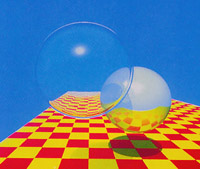
\includegraphics{early-raytracing-whitted}
    \centering
    \caption{Turner Whitted's original 1980 \cite{article:raytracing} image showing off the usage of ray tracing for
    reflection, refraction and shadows.}
    \label{fig:early-raytracing-whitted}
\end{figure}
Building upon ray tracing, an improved algorithm was published in 1986 by James T. Kajiya which used ray tracing
combined with a Monte Carlo algorithm in order to create a new algorithm that was called \emph{Monte
Carlo ray tracing} \cite{inproceedings:pathtracing}. Nowadays, Monte Carlo ray tracing is better
known as \emph{path tracing}.

It took another decade for path tracing to become the
physically based rendering approach that it is known for today. In 1996, Eric Lafortune improved
the algorithm by suggesting the usage of bidirectional path tracing \cite{techreport:pbr} and
finally the \ac{mlt} was suggested in 1997 by Eric Veach and Leonidas J. Guibas \cite{inproceedings:metropolis} to
improve performance in complex scenes.

This was the last notable improvement to the algorithm,
though many micro optimizations have since been published. All of these achievements and
improvements are generally collapsed into the term \emph{path tracing} since they do not diverge
from the general algorithm but instead improve upon it.

It took longer still for the industry to become interested in path tracing. The early interest in
ray tracing was of mostly academical and recreational nature. One of the most notable creations of
the early days of ray tracing is The Juggler created and published by Eric Graham in 1986
\cite{site:juggler} on an Amiga 1000. It was a pre-rendered animation using ray tracing. Eric Graham
stated that it took the Amiga 1 hour to render each frame \cite{site:juggler}.

\begin{figure}[H]
    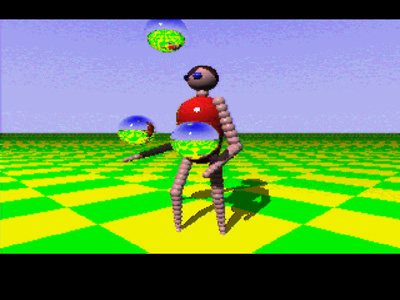
\includegraphics[scale=0.5]{amiga-juggler}
    \centering
    \caption{Eric Graham's Juggler}
    \label{fig:amiga-juggler}
\end{figure}
While the animation seems very primitive compared to the animations of today, it was exceptional at
the time. Ernie Wright's statement about The Juggler provides some contemporary context:

\blockquote[\cite{site:juggler}]{Turner Whitted's paper (1980) is widely regarded as the first modern
description of ray tracing methods in computer graphics. This paper's famous image of balls floating
above a checkerboard floor took 74 minutes to render on a DEC VAX 11/780 mainframe, a \$400,000
computer. The Juggler would appear a mere six years later, created and displayed on a \$2000 Amiga.}

The first feature-length computer-animated film,
\textit{Toy Story}, released in 1995 \cite{wiki:toy-story}, is sometimes miscredited as being the
first film using a ray tracing-like algorithm. However, it actually used traditional scanline
rendering. The first feature-length film using ray tracing, \textit{Cars}, was released much later,
in 2006 \cite{wiki:cars} \cite{inproceedings:cars} and started a wave of interest in the movie industry.

The first example of \emph{real time} path tracing was likely produced by the demo scene
\cite{wiki:demoscene} which was quick to adopt it \cite{site:realtime-radiosity-demos}
for the purpose of producing complex graphics rendered and generated on the fly. One notable
example of this is the WebGL Path Tracing by Evan Wallace made in 2010
\cite{site:webgl-path-tracing} which runs in most modern web browsers, making path tracing very
accessible.

\begin{figure}[H]
    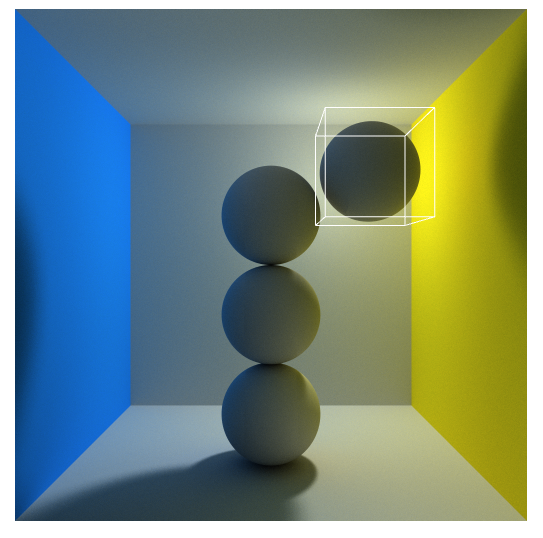
\includegraphics[scale=0.4]{webgl-pathtracer}
    \centering
    \caption{WebGL Path Tracer by Evan Wallace}
    \label{fig:webgl-pathtracer}
\end{figure}

Another example is the demo \textit{5 faces} by Fairlight from 2013
\cite{wiki:5faces-fairlight} which
uses a real time ray tracer running on the \acs{gpu} to render a complex scene at 30 \acs{fps}.

\begin{figure}[H]
    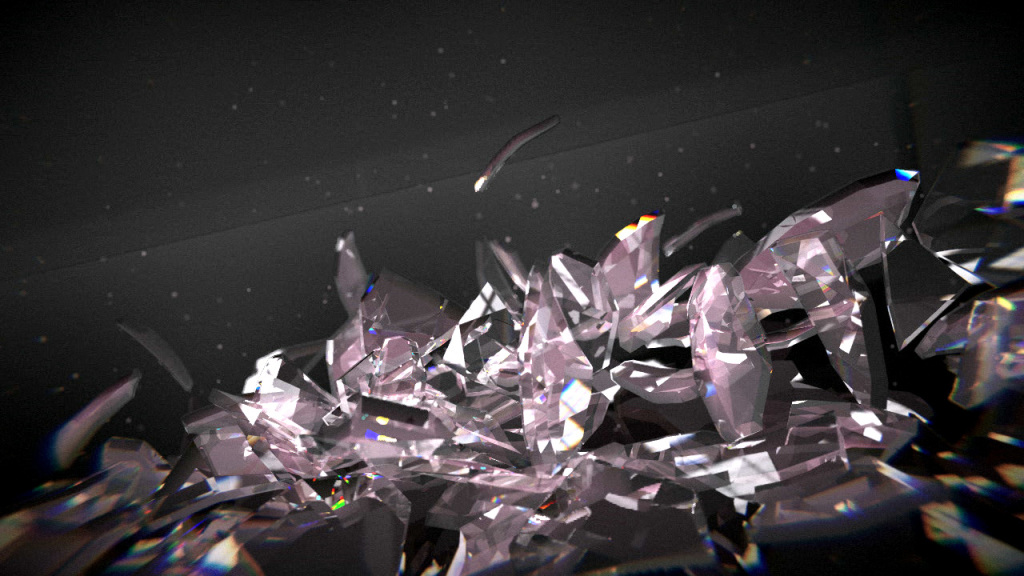
\includegraphics[scale=0.5]{5faces}
    \centering
    \caption{5 faces by Fairlight}
    \label{fig:5faces}
\end{figure}

In the past, some critics have offered critical insights about why it might not be a viable
alternative to rasterization on consumer hardware in the short term
\cite{site:raytracing-vs-rasterization} \cite{site:codinghorror-raytracing}. Even John Carmack of
id Software was sceptical of real time ray tracing in games in 2012 in a comment on Ars Technica
\cite{site:carmack-scepticism}.

\section{Current State of Technology}
Recently the interested in real time path tracing seems to be at peak levels. The most notable
example of this is Jacco Bikker's and Jeroen van Schijndel's \emph{Brigade Renderer} \cite{article:brigade}
\cite{site:brigade}. This renderer is aimed at game developers and is meant to run on commodity
hardware in real time. Its company, OTOY, is also developing a cloud-based rendering solution
called Octane Render \cite{site:octane} for animation professionals.

Microsoft's DirectX 12 \cite{site:dx12-raytracing} is receiving \emph{Hybrid Ray-Traced Shadows}, a
technology that combines real time ray tracing with rasterization to create fast high quality
shadows.

A video game using actual real time path tracing and physics called \emph{Sfera} was created by
David Bucciarelli \cite{site:sfera} in 2011. It uses OpenCL for calculating the paths and OpenGL to
render them to the screen.

It's important to keep in mind that while the real time graphics industry has mostly been driven by
video games, the most important hardware currently exist in game consoles which generally evolve at
a much slower pace than desktop computers in terms of hardware power and their graphics hardware
especially is usually non-upgradeable. This means that it wouldn't be economically viable to
develop a real time path tracing renderer that only ran on current generation desktop computers
because most consumers would not be able to benefit from the technology.

\chapter{Research}
\lipsum[1]

\section{Results}
\lipsum[1]

\section{Evaluation}
\lipsum[1]

\chapter{Conclusion}
\lipsum[1]

\section{Outlook}
\lipsum[1]

\listoffigures
 
\listoftables

\bibliographystyle{unsrt}
\bibliography{main}
    
\end{document}
